% ============================================================================
%  Benchmarking salarial - presentacion interna de ActuaLab, V2
%
%  COMPILAR:  pdflatex presentacion_v2.tex   (dos veces, para el indice)
%
%  QUE CAMBIA RESPECTO A LA V1 (`presentacion.tex`, que se conserva):
%
%  1. CONCEPTOS, NO CIFRAS. Cada lamina defiende UNA idea y la cifra es su
%     prueba, no su contenido. Regla: como mucho dos numeros por lamina, y solo
%     los que sostienen la idea del titulo. La tabla de nueve cifras del final
%     desaparece; quien las quiera tiene `mediciones.md`.
%
%  2. LA SECCION DE RESULTADOS SE REESCRIBE. La v1 contaba QUE se midio. Esta
%     cuenta QUE SE APRENDIO, que es lo que se recuerda: que cobertura y
%     precision son ganancias distintas, que un promedio bueno escondia un
%     defecto grave, y que la etiqueta de confianza era algebraicamente
%     incapaz de cambiar. Nada de eso estaba en la v1.
%
%  NO se citan codigos de decision (D-013, D-022...): son referencias internas
%  de `docs/registro_decisiones.md` y fuera de ese fichero no significan nada.
%
%  ESTILO: tema `Madrid` de beamer, de serie. Registro descriptivo y plano: se
%  enuncia la regla y la cifra, sin cerrar la lamina con una maxima.
% ============================================================================
\documentclass[11pt]{beamer}

\usepackage[utf8]{inputenc}
\usepackage[T1]{fontenc}
% Latin Modern: sin esto, `fontenc T1` cae a las Computer Modern de mapa de bits
% y el PDF sale con texto que no se puede buscar ni copiar.
\usepackage{lmodern}
\usepackage[spanish, es-noshorthands, es-nolists]{babel}
\usepackage{amsmath}
\usepackage{booktabs}
\usepackage{graphicx}
\graphicspath{{figuras/}}

\usetheme{Madrid}

\title[Agrupación de puestos]{Agrupación de puestos}
\subtitle{Cómo se construye el modelo, y qué se aprendió al medirlo}
\author[P. A. Encalada]{Pablo Andrés Encalada}
\institute[ActuaLab]{ActuaLab}
\date{\today}

\begin{document}

\begin{frame}[plain]
\titlepage
\end{frame}

\begin{frame}{Contenido}
\tableofcontents
\end{frame}

% ############################################################################
\section{El problema}
% ############################################################################

\begin{frame}{La dificultad está en el denominador}
\begin{itemize}
\item La referencia de mercado es una mediana. El cálculo no tiene dificultad.
\item La dificultad está en decidir \alert{quién entra} en esa mediana: qué
títulos de cargo son el mismo puesto.
\item Esa decisión es el modelo. Todo lo demás se deriva de ella.
\end{itemize}
\vspace{1em}
\begin{block}{La restricción}
La etiqueta de cargo es texto libre escrito por el cliente. No hay taxonomía de
referencia, y construir una obligaría a mapear a mano, que es lo que se quiere
evitar.
\end{block}
\end{frame}

\begin{frame}{El catálogo no está roto: está delgado}
\begin{itemize}
\item La etiqueta de cargo funciona. El problema no es que la gente escriba mal
lo que hace.
\item El problema es que \alert{casi ningún puesto tiene suficientes empresas
detrás}. La mediana de empresas por título es \alert{una}.
\end{itemize}
\vspace{0.8em}
Son dos diagnósticos distintos, y el tratamiento es distinto:
\begin{itemize}
\item Si estuviera roto semánticamente, haría falta otra representación.
\item Estando delgado, hace falta \textbf{tomar fuerza prestada} de puestos
vecinos.
\end{itemize}
\vspace{0.8em}
El segundo es un problema de estimación en áreas pequeñas, con literatura
propia. El primero habría sido un problema de clasificación.
\end{frame}

\begin{frame}{Espesor del catálogo de cargos}
\begin{figure}
\centering
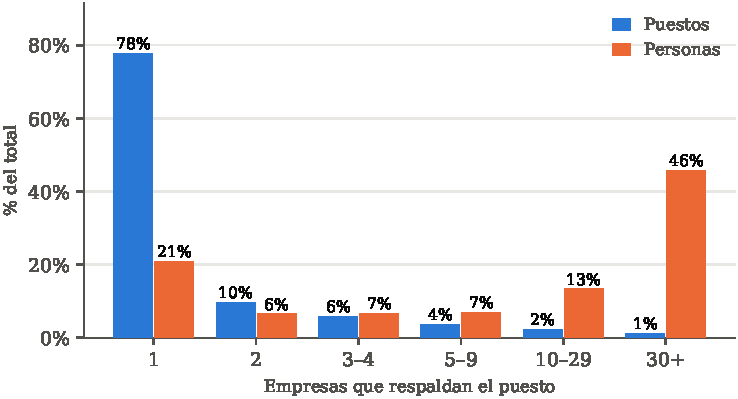
\includegraphics[width=0.92\linewidth]{espesor_catalogo.pdf}
\end{figure}
{\footnotesize Casi todos los puestos son delgados; casi toda la gente está en
los pocos que son gruesos.}
\end{frame}

\begin{frame}{Hay un techo, y saber dónde está cambia cómo se lee todo}
Dentro de un mismo cargo, el sueldo se separa por dos motivos: en qué empresa
trabaja la persona, y dónde cae dentro de esa nómina.
\vspace{0.8em}
\begin{itemize}
\item El primero pesa el doble que el segundo. \alert{La empresa explica el
81\,\%} de lo que no se puede predecir desde el puesto.
\item Eso no es un defecto del método: es información que \textbf{no está en el
título del cargo} y que ningún método basado en el puesto puede recuperar.
\end{itemize}
\vspace{0.8em}
Descontando ese suelo, el margen recuperable agrupando mejor es del orden del
\alert{12\,\%}.
\vspace{0.5em}

Cualquier resultado se lee contra ese número, no contra cero. Una mejora del
4\,\% es un tercio de todo lo disponible; una del 40\,\% está mal medida.
\end{frame}

\begin{frame}{Descomposición del error de predicción}
\begin{figure}
\centering
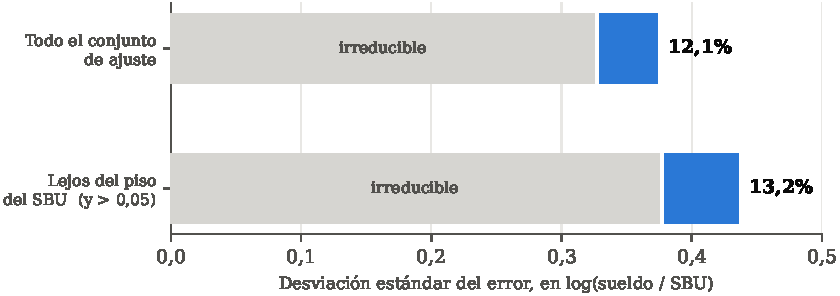
\includegraphics[width=0.90\linewidth]{descomposicion_error.pdf}
\end{figure}
{\footnotesize En color, la fracción del error atribuible al agrupamiento. El
resto lo genera el empleador.}
\end{frame}

% ############################################################################
\section{Cómo se agrupa}
% ############################################################################

\begin{frame}{Dos señales que no se sustituyen}
Juntar las grafías del mismo puesto necesita dos criterios, y cada uno es ciego
donde el otro ve:
\vspace{0.8em}
\begin{block}{El significado}
Une \texttt{ODONTOLOGA} con \texttt{DENTISTA}, que no comparten ni una letra en
el mismo sitio. Lo hace el \textit{embedding}.
\end{block}
\begin{block}{La ortografía}
Une \texttt{VENDEROR} con \texttt{VENDEDOR}. El \textit{embedding} \alert{no}
los une ---puntúan 0,72 frente a un umbral de 0,95--- porque aprendió qué
significan las palabras, y una errata no significa nada.
\end{block}
\vspace{0.6em}
Por eso son dos pasadas separadas, y no un criterio mezclado.
\end{frame}

\begin{frame}{El enemigo es la cadena, no el par malo}
Al agrupar por parecido, la regla ingenua es: si A se parece a B y B a C, los
tres al mismo grupo.
\vspace{0.8em}
\begin{itemize}
\item Medido, eso produce un grupo de \alert{1.758} títulos que contiene a la
vez \texttt{ASISTENTE CONTABLE} y \texttt{AUXILIAR DE LIMPIEZA}.
\item \textbf{Ningún par de esa cadena es absurdo.} El grupo entero sí.
\end{itemize}
\vspace{0.8em}
La regla que se usa exige que \alert{todos} los títulos de un grupo se parezcan
a todos los del otro. No basta un puente.
\vspace{0.8em}

Lo confirma un dato lateral: con esa regla, el cerrojo que impide unir niveles
jerárquicos distintos apenas se activa. El daño no venía de pares malos.
\end{frame}

\begin{frame}{Estar bien medido no es ser relevante}
Para un título que no está en la base se buscan puestos parecidos. La forma
ingenua de combinarlos es pesar por \emph{parecido} $\times$ \emph{precisión}.
\vspace{0.6em}
\begin{table}
\centering
\small
\begin{tabular}{lrr}
\toprule
Vecinos de \texttt{OPERADOR DE PARQUEADERO} & Parecido & Peso \\
\midrule
\texttt{OPERADOR DE PARQUEADEROS} & 0,99 & 8\,\% \\
\texttt{OPERADOR DE EXCAVADORA} & 0,83 & \alert{46\,\%} \\
\bottomrule
\end{tabular}
\end{table}
\vspace{0.6em}
El error es tratar las dos cosas como si fueran la misma. Un vecino
perfectamente medido que \textbf{no es tu puesto} no sirve, por muchos datos que
tenga. La precisión no compra relevancia.
\end{frame}

\begin{frame}{El ruido se promedia; el sesgo, no}
Cada vecino aporta dos incertidumbres distintas, y se combinan de forma
distinta:
\vspace{0.8em}
\begin{itemize}
\item \textbf{Su centro está mal medido.} Es ruido independiente: unos vecinos
fallan por arriba y otros por abajo, y al promediar veinticinco se cancela.
\item \textbf{No es tu puesto.} Es un \alert{sesgo compartido}: si los
veinticinco están igual de lejos, promediarlos no acerca la respuesta ni un
milímetro.
\end{itemize}
\vspace{0.8em}
\begin{block}{Por qué importa}
Tratando el segundo como si fuera ruido, un puesto \textbf{sin vecindario real}
salía con un intervalo estrecho, solo por haber promediado a mucha gente
equivocada. El modelo decía que estaba seguro porque tenía muchos datos, todos
irrelevantes.
\end{block}
\end{frame}

\begin{frame}{La consecuencia: el modelo sabe cuándo no sabe}
\texttt{LOTERO} no tiene vecinos de verdad. El \textit{embedding} se agarra a la
terminación \emph{-ero} y ofrece \texttt{LINIERO}, \texttt{BOTERO},
\texttt{TESORERO}. \texttt{TESORERO} paga dos veces y media más.
\vspace{1em}
Con la formulación anterior, y \textbf{sin ninguna regla especial}:
\begin{itemize}
\item todos los vecinos están lejos,
\item el término de sesgo domina y no se cancela al promediar,
\item el intervalo se dispara,
\item y la confianza cae a BAJA.
\end{itemize}
\vspace{0.8em}
No hay lista de excepciones ni casos particulares en el código. El caso
degenerado se delata solo.
\end{frame}

% ############################################################################
\section{Qué se aprendió al medir}
% ############################################################################

\begin{frame}{El instrumento funcionó contra nosotros}
El proyecto arrancó sobre una hipótesis: que la \textbf{composición del pago}
---fijo, comisiones, extras--- permitiría distinguir puestos dentro de una
etiqueta ancha.
\vspace{0.8em}
\begin{itemize}
\item Medida fuera de muestra, vale un \alert{0,2\,\%} sobre un techo del
12\,\%. Contra un placebo que da cero.
\item El eje que sí discrimina resultó ser el \textbf{nivel jerárquico}, que
nadie había medido.
\end{itemize}
\vspace{0.8em}
El protocolo se construyó \textbf{antes} que el modelo, y su primer resultado
fue falsificar la premisa del proyecto. La reformulación posterior ---de buscar
una covariable ausente a estimar en áreas pequeñas--- se deriva de ese rechazo.
\end{frame}

\begin{frame}{El nivel no solo mueve la media: escala la dispersión}
\begin{itemize}
\item Dentro de la misma empresa y la misma área, el escalón jerárquico explica
buena parte de lo que separa a dos personas con el mismo título. El placebo da
cero exacto.
\item Del escalón más bajo al más alto hay \alert{$2{,}11\times$} de sueldo.
\end{itemize}
\vspace{0.8em}
\begin{block}{Y un efecto que no se esperaba}
El escalón también multiplica por trece la \textbf{dispersión entre empresas}.
Un auxiliar de limpieza cobra casi lo mismo en todas partes ---el mínimo legal
comprime desde abajo--- y un gerente general no.

\vspace{0.3em}
Eso obliga a que la banda sea distinta por cargo, no un ancho fijo.
\end{block}
\end{frame}

\begin{frame}{La escalera de niveles}
\begin{figure}
\centering
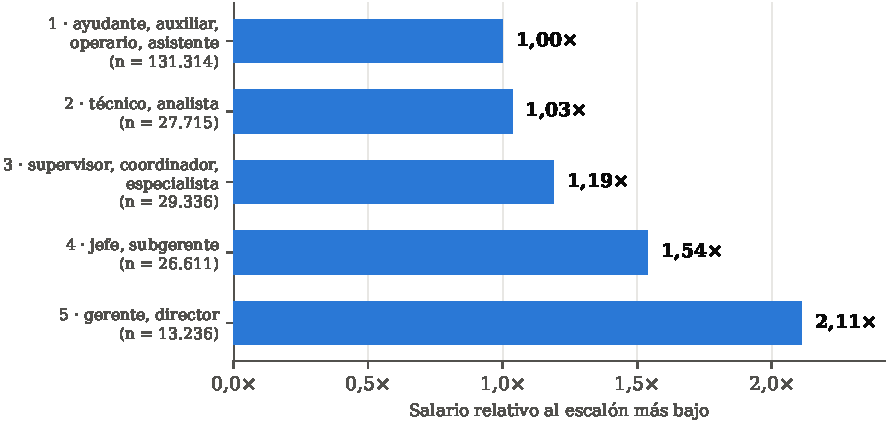
\includegraphics[width=0.86\linewidth]{escalera_niveles.pdf}
\end{figure}
{\footnotesize Salario relativo al escalón más bajo, estimado dentro de empresa
y área.}
\end{frame}

\begin{frame}{Cobertura y precisión son ganancias distintas}
Consolidar las grafías del mismo puesto \textbf{no mejora la precisión}: el
efecto sobre el error roza el cero.
\vspace{0.8em}
\begin{itemize}
\item Lo que mejora es \alert{a cuánta gente se le puede responder de primera
mano}, con los datos de su propia celda en vez de pidiendo prestado al
vecindario.
\item Siete grafías con una empresa cada una no estiman mejor por separado:
simplemente \textbf{ninguna llega al suelo}. Juntas, sí.
\end{itemize}
\vspace{0.8em}
\begin{block}{La lección de método}
Midiendo solo el error, esta mejora se habría descartado. Hay ganancias que no
aparecen en la métrica primaria, y hay que declarar la secundaria antes de
medir.
\end{block}
\end{frame}

\begin{frame}{Un promedio bueno escondía un defecto grave}
La banda promete contener a la mitad central de las empresas. Medida sobre
empresas apartadas, contenía al \alert{53\,\%}: aparentemente correcta.
\vspace{0.8em}
\begin{itemize}
\item Pero ese 53\,\% era el promedio de cargos donde contenía al \alert{18\,\%}
y cargos donde contenía al \alert{98\,\%}.
\item El defecto no era el ancho de la banda: era que \textbf{el ancho era el
mismo para todos los cargos}, cuando la dispersión no lo es.
\end{itemize}
\vspace{0.8em}
La cobertura media no lo detecta. Hace falta mirar el \textbf{recorrido} entre
grupos de cargos, que es donde el defecto se ve.
\vspace{0.5em}

Corregido, ese recorrido baja en un factor de doce.
\end{frame}

\begin{frame}{La etiqueta de confianza no podía cambiar}
Cada cifra sale con una marca de ALTA, MEDIA o BAJA. Al auditarla apareció esto:
\vspace{0.8em}
\begin{itemize}
\item La marca dependía de una cantidad que pesaba el \alert{0,1\,\%} de la
varianza. Los otros dos términos, que pesan el 99,9\,\%, son iguales para todas
las celdas.
\item Desarrollando el álgebra, salir de ALTA exigía menos empresas de las que
el suelo mínimo ya garantizaba. Era \alert{imposible por construcción}.
\end{itemize}
\vspace{0.8em}
Medido: \textbf{el 100,00\,\% de las celdas salía ALTA}. La más desfavorable de
toda la base no rozaba el corte.
\vspace{0.6em}

Reemplazada por la incertidumbre del propio centro, las tres marcas se reparten
y \textbf{predicen} cuánto se mueve la referencia: un 4\,\% en ALTA, un 13\,\%
en MEDIA, un 32\,\% en BAJA.
\end{frame}

\begin{frame}{Segmentar para estrechar y para corregir el centro no es lo mismo}
\begin{itemize}
\item Separar el mercado por tamaño de empresa \textbf{no estrecha la banda}: la
incertidumbre del centro sube más de lo que baja el ancho.
\item Pero el centro estaba \alert{sesgado}, y cada vez más cuanto más alto el
cargo. A una empresa pequeña se le decía que su gerente general cobraba muy por
debajo del mercado, cuando entre sus pares estaba bien.
\end{itemize}
\vspace{0.8em}
Son dos preguntas distintas sobre la misma segmentación, y la respuesta no es la
misma. El tamaño entra como desplazamiento del centro, y no como una partición
del mercado.
\end{frame}

\begin{frame}{Sesgo de nivel por tamaño de empresa}
\begin{figure}
\centering
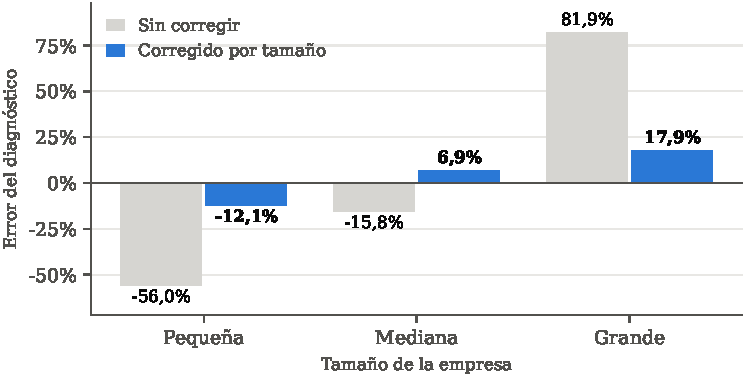
\includegraphics[width=0.78\linewidth]{sesgo_tamano.pdf}
\end{figure}
{\footnotesize El sesgo del centro casi desaparece al corregir por tamaño. La
banda, en cambio, no se estrecha.}
\end{frame}

\begin{frame}{El placebo es lo que separa la señal de la mecánica}
Cualquier reagrupación \textbf{mejora la cobertura por construcción}: al juntar
celdas hay más respaldo por celda, y las cifras se ven mejor. Eso no demuestra
que la regla esté eligiendo bien.
\vspace{0.8em}
\begin{block}{El contraste}
Se repite el experimento mandando \alert{las mismas fusiones a destinos elegidos
al azar}. Si el placebo mejora igual, la ganancia venía del mecanismo.
\end{block}
\vspace{0.8em}
En la fusión por errata, el placebo empeora el error en dos órdenes de magnitud
respecto a la regla real. Eso es lo que demuestra que la distancia de edición
elige bien el destino.
\vspace{0.5em}

En otro experimento el placebo \textbf{seleccionó más cargos que la señal real},
y bastó para descartar el método.
\end{frame}

% ############################################################################
\section{Qué se puede prometer}
% ############################################################################

\begin{frame}{El alcance, dicho con precisión}
\begin{itemize}
\item Lo que se entrega es el \alert{mercado}: qué paga el conjunto de empresas
por un puesto. No la política salarial de una empresa concreta, que es donde
vive el 81\,\% de la variación.
\item El sistema \textbf{responde siempre}. Un cliente sin referencia no se
queda quieto: se inventa un número. Por eso se responde, y por eso la marca de
confianza tiene que ser real.
\item Cada decisión de método está registrada con su evidencia, sus
alternativas y su criterio declarado antes de medir.
\end{itemize}
\vspace{1em}
\begin{block}{Lo que todavía no se puede decir}
Todo lo reportado sale de particiones de validación dentro del conjunto de
ajuste. Es consistencia interna, no validación externa: el conjunto de
evaluación final se reserva para una sola pasada, al congelar el método.
\end{block}
\end{frame}

\end{document}
